\documentclass{exam}
\usepackage{algpseudocode}
\usepackage{algorithm}
\usepackage{amsmath}

\usepackage{indentfirst}
\usepackage{graphicx}
\usepackage{listings}
\usepackage{color}
\usepackage{fancyvrb}

\definecolor{mygreen}{rgb}{0,0.6,0}
\definecolor{mygray}{rgb}{0.5,0.5,0.5}
\definecolor{mymauve}{rgb}{0.58,0,0.82}

\lstset{ %
	backgroundcolor=\color{white},		% choose the background color; you must add \usepackage{color} or \usepackage{xcolor}
	basicstyle=\small\ttfamily,		% the size of the fonts that are used for the code
	breakatwhitespace=false,			% sets if automatic breaks should only happen at whitespace
	breaklines=true,					% sets automatic line breaking
	captionpos=b,						% sets the caption-position to bottom
	columns=fullflexible,
	commentstyle=\color{mygreen},		% comment style
	deletekeywords={...},				% if you want to delete keywords from the given language
	escapeinside={\%*}{*)},			% if you want to add LaTeX within your code
	extendedchars=true,				% lets you use non-ASCII characters; for 8-bits encodings only, does not work with UTF-8
	frame=single,						% adds a frame around the code
	keepspaces=true,					% keeps spaces in text, useful for keeping indentation of code (possibly needs columns=flexible)
	keywordstyle=\color{blue},			% keyword style
	language=Octave,					% the language of the code
	morekeywords={*,...},				% if you want to add more keywords to the set
	%   numbers=left,						% where to put the line-numbers; possible values are (none, left, right)
	%   numbersep=6pt,						% how far the line-numbers are from the code
	%   numberstyle=\tiny\color{mygray},	% the style that is used for the line-numbers
	rulecolor=\color{black},			% if not set, the frame-color may be changed on line-breaks within not-black text (e.g. comments (green here))
	showspaces=false,					% show spaces everywhere adding particular underscores; it overrides 'showstringspaces'
	showstringspaces=false,			% underline spaces within strings only
	showtabs=false,					% show tabs within strings adding particular underscores
	stepnumber=1,						% the step between two line-numbers. If it's 1, each line will be numbered
	stringstyle=\color{mymauve},		% string literal style
	tabsize=2,							% sets default tabsize to 2 spaces
	title=\lstname						% show the filename of files included with \lstinputlisting; also try caption instead of title
}

% Creates a new command to include a perl script, the first parameter is the filename of the script (without .pl), the second parameter is the caption
\newcommand{\octavescript}[2]{
	\lstinputlisting[caption=#2]{#1}
}

\newcommand{\MNLab}{Laborator\ \#6}
\newcommand{\MNLabTitle}{Soluția ecuației neliniare $f(x)=0$. Analiza convergenței. Lucrul cu polinoame în MATLAB. Rezolvarea sistemelor de ecuații neliniare.}
\newcommand{\MNLabTitleHeader}{Ecuații neliniare}
\newcommand{\MNAuthor}{Andrei STAN, Sorin Ciolofan}

\renewcommand{\contentsname}{Cuprins}
\renewcommand{\figurename}{Figura}
\renewcommand{\refname}{Referințe}

\setlength{\parskip}{0.5\baselineskip}

\graphicspath{{./img/}}

\title{
	\textmd{\textbf{\MNLabTitle}}
	\author{}
    \date{}
}

\pagestyle{headandfoot}

\header{Metode Numerice}
{\MNLabTitleHeader, Pagina \thepage\ din \numpages}
{2025}
\footer{Facultatea de Automatică și Calculatoare}{}{Pagina \thepage\ din \numpages}

\begin{document}

\begin{coverpages}

	\maketitle
	\tableofcontents

\end{coverpages}

\section{Obiective laborator}
În urma parcurgerii acestui laborator, studentul va fi capabil să:
\begin{itemize}
	\item determine aproximativ soluţiile unei ecuaţii neliniare;
	\item rezolve iterativ un sistem de ecuaţii neliniare;
        \item aplice metoda gradientului conjugat;
	\item lucreze în Octave cu polinoame.
\end{itemize}

\section{Noțiuni teoretice}

\subsection{Soluţia ecuaţiei neliniare $f(x) = 0$}

\subsubsection{Metode bazate pe interval}

Se porneşte de la observaţia că, dacă semnul unei funcții continue se modifică între punctele a şi b, $a < b$ atunci trebuie să existe un punct c, $a < c < b$ 
 astfel încât $f(c) = 0$. Se micşorează acest interval care încadrează rădăcina până ce se ajunge la o anumită precizie dorită.

\textbf{Metoda bisecţiei}. Dacă o funcţie îşi schimbă semnul pe un interval, adică $f(a)\cdot f(b)<0$, atunci se evaluează valoarea funcţiei în punctul de mijloc al intervalului, $c = \frac{a + b}{2}$. Dacă  $f(c)\cdot f(b)<0$ atunci rădăcina se află în intervalul $(c, b)$ unde se continuă căutarea. La fel, dacă  $f(c)\cdot f(a)<0$ atunci rădăcina se află în intervalul $(a, c)$. Procedura se repetă până ce se obţin estimări mai precise ale rădăcinii.

Se poate defini eroarea relativă procentuală folosind relaţia:
$$\epsilon=\left | \frac{x_{r}^{new}-x_{r}^{old}}{x_{r}^{new}} \right |$$

Când $\epsilon < tol$, algoritmul iterativ se termină, iar $x_{r}^{new}$ este considerată valoarea calculată a rădăcinii. Metoda aceasta este întotdeauna convergentă deoarece aplicarea repetată a algoritmului duce la o estimare mai precisă a rădăcinii.

Un alt avantaj al acestei metode este faptul că pentru o eroare acceptată $tol$, se poate calcula numărul maxim de iteraţii ce trebuie parcurse pentru a se ajunge la aproximarea dorită a rădăcinii, conform formulei:
$$n=\log_{2}(\frac{b-a}{tol}).$$

Algoritmul poate fi gândit ca o căutare binară a rădăcinii într-un vector cu $\frac{b-a}{tol}$ elemente, de unde și complexitatea.
    
\begin{algorithm}[H]
    \caption{Metoda Bisecției}
    \begin{algorithmic}[1]
        \State $i \gets 1$
        \While{$|f(c)| < \text{tol}$}
            \State $c \gets \frac{a + b}{2}$
            \If{$f(a) \cdot f(c) < 0$}
                \State $b \gets c$
            \Else
                \State $a \gets c$
            \EndIf
            \State $i \gets i + 1$
        \EndWhile
        \State \Return $c$
    \end{algorithmic}
\end{algorithm}

\subsubsection{Metode care nu se bazează pe un interval}

Este suficientă cunoaşterea unei valori iniţiale $x_i$ care este folosită mai departe pentru estimarea valorii următoare $x_{i+1}$. Aceste metode, spre deosebire de primele, pot fi convergente sau pot fi divergente. Atunci când ele converg, convergenţa este mult mai rapidă decât în cazul metodelor bazate pe interval.

\textbf{Metoda tangentei}. După cum s-a menţionat anterior, se porneşte cu o valoare de început $x_{i}$, apoi se deduce o estimare îmbunătăţită $x_{i+1}$. În cazul metodei tangentei, se duce o tangentă la curba din punctul de coordonate $[x_{i}, f(x_{i})]$. Punctul de intersecţie a tangentei cu $Ox$ se consideră  $x_{i+1}$. Această metodă nu are garanția convergenței, existând pericolul, printre altele, de a ajunge într-un punct extrem unde $f'(x) = 0$ sau în apropierea unuia. În spatele acestei metode se află de fapt aproximări succesive ale funcției date cu polinoame de gradul I.

Relaţia de recurenţă este:
$$x_{i+1}=x_{i}-\frac{f(x_{i})}{f^{'}(x_{i})}$$

Se poate arăta prin dezvoltare în serie Taylor că eroarea la iteraţia curentă este proporţională cu pătratul erorii la iteraţia precedentă \cite{Quad}, ceea ce, aproximativ, înseamnă că la fiecare iteraţie numărul de zecimale corect calculate din rădăcină se dublează:

Definim eroarea ca $e_k = x_k - x^*$, astfel încât $x_k = e_k + x^*$. Aplicând Teorema lui Taylor, pentru $x = x_k$ și $h = -e_k$, avem:

$$ f(x_k - e_k) = f(x_k) - e_k f'(x_k) + \frac{(e_k)^2}{2} f''(\xi_k) $$

pentru un $\xi_k$ situat între $x_k$ și $x^*$. Deoarece $x_k - e_k = x^*$ și $f(x^*) = 0$, obținem:

$$ 0 = f(x_k) - (x_k - x^*) f'(x_k) + \frac{(e_k)^2}{2} f''(\xi_k). $$

Cum derivata $f'$ este continuă și $f'(x^*) \neq 0$, avem $f'(x_k) \neq 0$ pentru $x_k$ suficient de aproape de $x^*$. Putem împărți ecuația la $f'(x_k)$:

$$ 0 = \frac{f(x_k)}{f'(x_k)} - (x_k - x^*) + \frac{(e_k)^2 f''(\xi_k)}{2 f'(x_k)}. $$

Prin definiția metodei lui Newton, rezultă:

$$ x_{k+1} - x^* = \frac{(e_k)^2 f''(\xi_k)}{2 f'(x_k)}. $$

Prin urmare,

$$ |x_{k+1} - x^*| \leq \left| \frac{f''(\xi_k)}{2 f'(x_k)} \right| e_k^2. $$

Prin continuitate, $f'(x_k)$ converge către $f'(x^*)$, iar cum $\xi_k$ este între $x_k$ și $x^*$, acesta converge către $x^*$, deci $f''(\xi_k)$ converge către $f''(x^*)$. Astfel, pentru $k$ suficient de mare,

$$ |x_{k+1} - x^*| \leq M |x_k - x^*|^2, \quad \text{unde} \quad M > \left| \frac{f''(x^*)}{2 f'(x^*)} \right|. $$

\begin{algorithm}[H]
    \caption{Metoda Tangentei (Newton)}
    \begin{algorithmic}[1]
        \State $i \gets 1$
        \While{$i \leq \text{max\_iter}$}
            \State $x_1 \gets x_0 - \frac{f(x_0)}{f'(x_0)}$
            \If{$|x_1 - x_0| < \text{tol}$}
                \State \textbf{break}
            \EndIf
            \State $x_0 \gets x_1$
            \State $i \gets i + 1$
        \EndWhile
        \State \Return $x_1$
    \end{algorithmic}
\end{algorithm}

\textbf{Metoda secantei}. De multe ori nu se poate calcula derivata funcțiilor neliniare, de aceea tangenta se aproximează prin secanta care trece prin două puncte apropiate. Astfel $x_i$ devine:
$$x_{i+1}=x_i - \frac{f(x_i)(x_i - x_{i - 1})}{f(x_i)-f(x_{i - 1})}.$$


\begin{algorithm}[H]
    \caption{Metoda Secantei}
    \begin{algorithmic}[1]
        \State $i \gets 1$
        \While{$i \leq \text{max\_iter}$}
            \State $x_2 \gets x_1 - \frac{f(x_1)(x_1 - x_0)}{f(x_1) - f(x_0)}$
            \If{$|x_2 - x_1| < \text{tol}$}
                \State \textbf{break}
            \EndIf
            \State $x_0 \gets x_1$
            \State $x_1 \gets x_2$
            \State $i \gets i + 1$
        \EndWhile
        \State \Return $x_2$
    \end{algorithmic}
\end{algorithm}

\subsubsection{Viteza de convergență a metodelor prezentate}

În tabelul de mai jos se observă numărul de iterații prin care a trecut fiecare metodă pentru a aproxima rădăcina unei funcții neliniare. Valoarea toleranței alese a fost $10^{-15}$. Ca valori inițiale, pentru o rădăcină $c$, au fost alese fie valorile $[[c], [c] + 1]$ în cazul metodelor ce necesită două valori inițiale, fie $[c] + 1$ în cazul celor cu o singură valoare inițială, unde $[c]$ reprezintă partea întreagă a numărului $c$.

Se poate observa creșterea în eficiență de la metoda bisecției la următoarele două, care au avut de departe cel mai mic număr de iterații. De asemenea, metoda contracției depinde foarte mult de funcția $g(x)$ pentru viteza de convergență: în cazurile în care $|g'(x) | >= 1$ aceasta nu converge, așa cum se vede pentru ultima funcție. Între metoda tangentei și cea a secantei prima se dovedește mai rapidă datorită formulelor exacte ale derivatelor funcțiilor. Cea din urmă este totuși mai versatilă, fiind aplicabilă și în cazurile în care derivata funcției neliniare nu este cunoscută.

\begin{table}[h]
\centering
\label{tab:root_finding}
\begin{tabular}{lccc}
\textbf{Funcție} & \textbf{Bisecție} & \textbf{Secantă} & \textbf{Tangentă}\\
$0.25e^x - 2$ & 48 & 7 & 7 \\
$3\cos(x) - 4x$ & 50 & 7 & 5 \\
$x^2 - 2$ & 49 & 7 & 6\\
$\ln(x) - 2$ & 46 & 6 & 4\\
$ x^2 + \sqrt{x}- 6$ & 48 & 7 & 5 \\
\end{tabular}
\caption{Numărul iterațiilor necesare pentru fiecare metoda}
\end{table}
\subsection{Metoda Gradientului Conjugat și a Pașilor Descrescători}

Pentru sisteme de forma $Ax=b$, dacă matricea $A$ este pozitiv semidefinită și simetrică, putem utiliza atât metoda pașilor descrescători, cât și metoda gradientului conjugat pentru a ajunge la soluția $x$. 
Ambele metode au în spate forma pătratică a matricei $A$:
$$f(x)=\frac{1}{2}x^TAx-b^Tx+c$$
Gradientul unei forme pătratice este definit ca fiind:
$$\nabla f(x) = 
\begin{bmatrix}
\frac{\partial}{\partial x_1} f(x) \\
\frac{\partial}{\partial x_2} f(x) \\
\vdots \\
\frac{\partial}{\partial x_n} f(x)
\end{bmatrix}
$$
Prin aplicarea gradientului pe forma pătratică se ajunge la ecuația următoare:
$$\nabla f(x) = \frac{1}{2} A^T x + \frac{1}{2} A x - b$$

Datorită faptului că matricea $A$ este simetrică $A = A^T$, așadar ecuația devine:
$$\nabla f(x) = Ax-b$$

Când $\nabla f(x) = 0$ reiese ecuația inițială $Ax=b$, așadar vectorul $x$ care îndeplinește acest criteriu, deci care minimizează forma pătratică, este soluția sistemului inițial.


\subsubsection{Metoda pașilor descrescători} 

Ase bazează pe aproximări succesive, de fiecare dată "pasul" este efectuat astfel încât $f(x)$ să "scadă" cel mai rapid, cu alte cuvinte sensul vectorului ales este cel opus lui $\nabla f(x)$. De asemenea, două direcții succesive sunt ortogonale. Deoarece $\nabla f(x) = Ax-b$, sensul vectorului ales (care se numește reziduu) are formula $r^{(k)} = b - Ax^{(k)}$.

La fiecare pas al algoritmului se calculează $x^{(k)}$, acesta fiind
$$x^{(k)} = x^{(k-1)} + \alpha r^{(k-1)}$$ 

Deoarece pași succesivi sunt efectuați pe direcții ortogonale:

\begin{align*}
r^{(k + 1)T} r^{(k)} &= 0 \\
(b - Ax^{(k)})^T r^{(k)} &= 0 \\
(b - A(x^{(k)} + \alpha r^{(k)}))^T r^{(k)} &= 0 \\
(b - Ax^{(k)T}) r^{(k)} - \alpha (Ar^{(k)T}) r^{(k)} &= 0 \\
(b - Ax^{(k)T}) r^{(k)} &= \alpha (Ar^{(k)T}) r^{(k)} \\
r^{(k)T} r^{(k)} &= \alpha r^{(k)T} (Ar^{(k)}) \\
\alpha &= \frac{r^{(k)T} r^{(k)}}{r^{(k)T} Ar^{(k)}}
\end{align*}

Pentru a nu calcula de fiecare dată $r^{(k)} = b - Ax^{(k)}$ se poate înmulți ecuația $x^{(k)} = x^{(k-1)} + \alpha r^{(k-1)}$ la stânga cu $-A$. În urma acestei operații se ajunge la formula $$r^{(k+1)} = r^{(k)} - \alpha Ar^{(k)}$$
\begin{figure}[H]
	\centering
	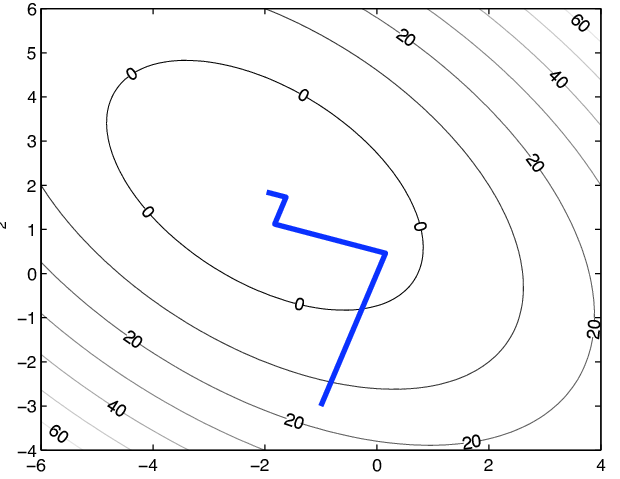
\includegraphics[width=0.5\textwidth]{lab6/img/steepest_descent.png}
	\caption{Metoda Pașilor Descrescători}
	\label{fig:1}
\end{figure}

\begin{algorithm}[H]
    \caption{Metoda Pașilor Descrescători}
    \begin{algorithmic}[1]
        \State $r_0 \gets b - A \cdot x_0$ \Comment{Calculăm reziduul inițial}
        \State $i \gets 1$
        \While{$i \leq \text{max\_iter}$}
            \State $\alpha_i \gets \frac{r_i^T r_i}{r_i^T A r_i}$ \Comment{Calculăm pasul de învățare}
            \State $x_{i+1} \gets x_i + \alpha_i \cdot r_i$ \Comment{Actualizăm soluția}
            \State $r_{i+1} \gets r_i - \alpha_i \cdot A \cdot r_i$ \Comment{Actualizăm reziduul}
            \If{$\|r_{i+1}\| < \text{tol}$}
                \State \textbf{break}
            \EndIf
            \State $i \gets i + 1$
        \EndWhile
        \State \Return $x_{i+1}$
    \end{algorithmic}
\end{algorithm}

\subsubsection{Metoda Gradientului Conjugat}

O metodă mult mai eficientă este cea a gradientului conjugat, ea având proprietatea de a converge garantat după cel mult $n$ iterații. Ideea din spatele acestei metode este de a construi un set de direcții de căutare conjugate între ele în raport cu matricea $A$. Spre deosebire de metoda pașilor descrescători, unde fiecare direcție de căutare este ortogonală cu cea anterioară, în metoda gradientului conjugat direcțiile sunt $A-conjugate$, adică satisfac relația:

$$
p^{(i)T} A p^{(j)} = 0, \quad \text{pentru } i \neq j.
$$

Această proprietate asigură că soluția exactă este atinsă în cel mult $n$ pași pentru un sistem de dimensiune $n$, în cazul în care nu există erori numerice.

Algoritmul începe similar cu metoda pașilor descrescători, însă în loc să folosească doar $r^{(k)}$ ca direcție de căutare, se construiește un nou vector $p^{(k)}$, care combină reziduul curent cu direcția anterioară:

$$
p^{(k)} = r^{(k)} + \beta^{(k)} p^{(k-1)}
$$

unde coeficientul $\beta^{(k)}$ este ales astfel încât direcțiile să rămână A-conjugate:

$$
\beta^{(k)} = \frac{r^{(k)T} r^{(k)}}{r^{(k-1)T} r^{(k-1)}}.
$$
Vectorii $p$ formează de fapt ceea ce se numește un subspațiu Krylov.
La formula lui $\beta$ se ajunge astfel:
$$ p^{(k)T} A p^{(k-1)} = 0 $$
$$ (r^{(k)} + \beta ^{(k)}p^{(k-1)})^T A p^{(k-1)} = 0 $$
$$ r^{(k)T} A p^{(k-1)} + \beta ^{(k)}p^{(k-1)T} A p^{(k-1)} = 0 $$
$$\beta^{(k)} = -\frac{\mathbf{r}^{(k)T} A \mathbf{p}^{(k-1)}}{\mathbf{p}^{(k-1)T} A \mathbf{p}^{(k-1)}}
$$
Folosim relația de actualizare a reziduului:
$$\mathbf{r}^{(k)} = \mathbf{r}^{(k-1)} - \alpha^{(k-1)} A \mathbf{p}^{(k-1)}$$
Așadar:
$$A \mathbf{p}^{(k-1)} = \frac{1}{\alpha^{(k-1)}} (\mathbf{r}^{(k-1)} - \mathbf{r}^{(k)}).
$$

$$\mathbf{r}^{(k) T} A \mathbf{p}^{(k-1)} = \frac{1}{\alpha^{(k-1)}} \mathbf{r}^{(k) T} (\mathbf{r}^{(k-1)} - \mathbf{r}^{(k)}) = -\frac{1}{\alpha^{(k-1)}} \mathbf{r}^{(k) T} \mathbf{r}^{(k)}
$$

deoarece $\mathbf{r}^{(k)}$ și $\mathbf{r}^{(k-1)}$ sunt ortogonale prin construcție.

$$\mathbf{p}^{(k-1) T} A \mathbf{p}^{(k-1)} = (\mathbf{r}^{(k-1)} + \beta^{(k-1)} \mathbf{p}^{(k-2)})^{T} A \mathbf{p}^{(k-1)}.
$$

$$\mathbf{p}^{(k-1) T} A \mathbf{p}^{(k-1)} = \frac{1}{\alpha^{(k-1)}} \mathbf{r}^{(k-1) T} (\mathbf{r}^{(k-1)} - \mathbf{r}^{(k)}) = \frac{1}{\alpha^{(k-1)}} \mathbf{r}^{(k-1) T} \mathbf{r}^{(k-1)}.
$$

Astfel, înlocuind numitorul și numărătorul se ajunge la formula generală a lui $\beta$.
În continuare, formula cu ajutorul căreia se determină pasul optim $\alpha^{(k)}$ pe direcția $p^{(k)}$:

$$
\alpha^{(k)} = \frac{r^{(k)T} r^{(k)}}{p^{(k)T} A p^{(k)}}.
$$

Noua aproximare $x^{(k+1)}$ și noul reziduu $r^{(k+1)}$ sunt actualizate astfel:

$$
x^{(k+1)} = x^{(k)} + \alpha^{(k)} p^{(k)}
$$
$$
r^{(k+1)} = r^{(k)} - \alpha^{(k)} A p^{(k)}.
$$

\begin{algorithm}[H]
    \caption{Metoda Gradientului Conjugat}
    \begin{algorithmic}[1]
        \State $r_0 \gets b - A \cdot x_0$ \Comment{Calculăm reziduul inițial}
        \State $p_0 \gets r_0$ \Comment{Direcția inițială}
        \State $i \gets 1$
        \While{$i \leq \text{max\_iter}$}
            \State $\alpha_i \gets \frac{r_i^T r_i}{p_i^T A p_i}$ \Comment{Calculăm pasul de învățare}
            \State $x_{i+1} \gets x_i + \alpha_i \cdot p_i$ \Comment{Actualizăm soluția}
            \State $r_{i+1} \gets r_i - \alpha_i \cdot A \cdot p_i$ \Comment{Actualizăm reziduul}
            \If{$\|r_{i+1}\| < \text{tol}$}
                \State \textbf{break}
            \EndIf
            \State $\beta_{i+1} \gets \frac{r_{i+1}^T r_{i+1}}{r_i^T r_i}$ \Comment{Calculăm coeficientul de actualizare}
            \State $p_{i+1} \gets r_{i+1} + \beta_{i + 1} \cdot p_i$ \Comment{Actualizăm direcția conjugată}
            \State $i \gets i + 1$
        \EndWhile
        \State \Return $x_{i+1}$
    \end{algorithmic}
\end{algorithm}

Comparativ cu metoda pașilor descrescători, metoda gradientului conjugat converge mult mai rapid, mai ales pentru sisteme mari și rare, ceea ce o face una dintre cele mai eficiente metode iterative pentru rezolvarea sistemelor de ecuații liniare cu matrice simetrică și pozitiv semidefinită.
\begin{figure}[H]
	\centering
	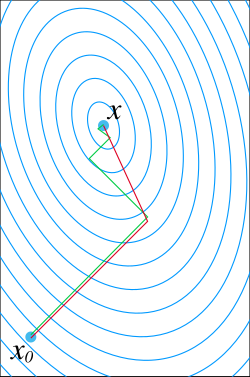
\includegraphics[width=0.3\textwidth]{lab6/img/conjugate_vs_steepest.png}
	\caption{Metoda Gradientului Conjugat și a Pașilor descrescători}
	\label{fig:1}
\end{figure}

\subsection{Sisteme de ecuații neliniare}
Un sistem de ecuaţii neliniare are forma:

$$\left\{
	\begin{array}{lll}
		f_{1}(x_{1},x_{2},x_{3},...,x_{n-1},x_{n})=0 \\
		f_{2}(x_{1},x_{2},x_{3},...,x_{n-1},x_{n})=0 \\
		...                                          \\
		f_{n}(x_{1},x_{2},x_{3},...,x_{n-1},x_{n})=0 \\
	\end{array}
	\right.$$

\noindent  unde $f_{i}$ reprezintă funcţii cunoscute de $n$ variabile $x_{1}, x_{2}, ..., x_{n}$, presupuse continue, împreună cu derivatele lor parţiale până la un ordin convenabil (de obicei, până la ordinul doi). Se va urmări găsirea soluţiilor reale ale sistemului într-un anumit domeniu de interes, domeniu în care se consideră valabile proprietăţile de continuitate impuse funcţiilor $f_{i}$ şi derivatelor lor. Rezolvarea sistemului este un proces iterativ în care se porneşte de la o aproximaţie iniţială pe care algoritmul o va îmbunătăţi până ce se va îndeplini o condiţie de convergenţă. În cazul de faţă, localizarea apriori a soluţiei nu mai este posibilă (nu există o metodă analoagă metodei înjumătăţirii intervalelor).

\textit{Metoda Newton}

Pentru simplificarea notaţiei, considerăm $F=\left(\begin{array}{c}f_{1}\\f_{2}\\f_{3}\\...\\f_{n} \end{array}\right)$ şi $x=(x_{1},x_{2},...,x_{n})$. Sistemul îl putem rescrie ca $F(x)=0$.
Notăm cu $x^{(k)}$ estimarea la pasul $k$ a soluţiei $x^{*}$, deci $F(x^{*})=0$.

Se poate deduce relaţia:
$$x^{(k+1)} = x^{(k)} - J(x^{(k)})^{-1}F(x^{(k)}), k=0,1,2,... $$

\noindent  unde $J$ este matricea \textit{Jacobiană}
\[J=  \left( \begin{array}{ccc}
			\frac{\partial F_{1}}{ \partial x_{1}} & ...   & \frac{\partial F_{1}}{ \partial x_{n}} \\
			{...}                                  & {...} & {...}                                  \\
			\frac{\partial F_{n}}{ \partial x_{1}} & ...   & \frac{\partial F_{n}}{ \partial x_{n}}
		\end{array} \right)\]

Dacă matricea $J$ este neinversabilă, atunci pasul este nedefinit. Vom presupune că $J(x^*)$ este inversabilă, iar continuitatea lui $J$ va asigura că $J(x^{(k)})$ este inversabilă pentru orice $x^{(k)}$ suficient de apropiat de $x^*$.
Secvenţa definită iterativ converge spre soluția $x^*$.
Condiţia de oprire la iteraţia $k$, $\left \|x^{*}-x^{(k)}  \right \|<tol$, unde $tol$ este o toleranţă dată, se poate arăta că revine la $\left \|x^{(k)}-x^{(k-1)}  \right \|<tol.$

\subsection{Polinoame}

\subsubsection{Rădăcinile polinoamelor}

Fie $p$ un polinom de grad $n$, $p(x)= a_{n}x^{n}+a_{n-1}x^{n-1}+a_{n-2}x^{n-2}+...+a_{1}x+a_{0}, \: cu \: a_{n}\neq 0$.
Conform cu \textit{teorema fundamentală a algebrei}, polinomul $p$ are $n$ rădăcini reale sau complexe (numărând şi multiplicităţile). În cazul în care coeficienţii $a_{i}$ sunt toţi reali,  rădăcinile complexe apar conjugate (de forma $c+id$ şi $c-id$).

Folosind regula semnelor a lui Descartes, putem număra câte rădăcini reale pozitive are polinomul $p$. Fie $v$ numărul variaţiilor de semn ale coeficienţilor $a_{n}, a_{n-1}, a_{n-2},.., a_{1},a_{0}$, ignorând coeficienţii care sunt nuli. Fie $n_{p}$ numărul de rădăcini pozitive. Avem următoarele două relaţii:

1) $n_{p}\leq v;$

2) $v-n_{p}$ este un număr par.

Analog, numărul de rădăcini reale negative ale lui $p(x)$ se obţine folosind numărul de schimbări de semn ale coeficienţilor polinomului  $p(-x)$.
Pentru determinarea rădăcinilor, se pot aplica metodele descrise anterior la punctul $b)$, dacă nu se cunoaşte localizarea rădăcinilor pe intervale.

\subsubsection{Lucrul cu polinoame în MATLAB}

În MATLAB, un polinom este reprezentat prin coeficienţii săi (în ordine descrescătoare). Vectorul \verb|p = [-2, -1, 0, 1, 2]| reprezintă polinomul $-2x^{4}-x^{3}+x+2$.

\textbf{Funcții MATLAB}
\begin{itemize}
    \item \verb|polyval(p, x)| - calculează $p(x)$.
    \item \verb|conv(p, q)| - calculează convoluția celor două polinoame (le înmulțește).
    \item \verb|polyder(p)| - calculează derivata polinomului.
    \item \verb|polyiny(p)| - calculează integrala polinomului.
\end{itemize}

\section{Probleme propuse}

\subsection{Problema 1}
Să se determine tipul (dacă sunt reale pozitive sau negative, complexe) rădăcinilor polinomului $p(x)=3x^{6}+x^{4}-2x^{3}-5$.
%\end{Problem}

\subsection{Problema 2}
Să se scrie în Octave un program care rezolvă un sistem de ecuaţii neliniare prin metoda Newton. Ca intrare, se consideră un vector coloană care reprezintă $x^{(0)}$, un pointer (handler) la o funcţie care evaluează $F$ într-un vector generic $x$, un pointer la o funcţie care calculează Jacobiana într-un vector generic $x$, o toleranţă dată $\epsilon$. Metoda se opreşte atunci când  $\left \| x^{(k)}-x^{(k-1)} \right \|< \epsilon$ şi returnează vectorul soluţie $x^{*}$ şi numărul de iteraţii $n$ care au fost necesare pentru producerea soluţiei.
%\end{Problem}
\bibliographystyle{plain}
\bibliography{refs}
\end{document}
